\documentclass[tikz,border=6pt]{standalone}
\usepackage{amsmath,amssymb}
\begin{document}
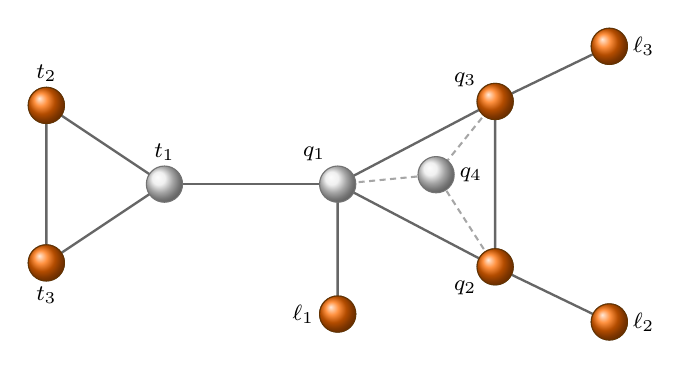
\begin{tikzpicture}[
  v/.style={circle,shading=ball,ball color=white!92!black,draw=black!55,minimum size=4.6mm,inner sep=0pt},
  d/.style={v,ball color=orange!85!red,draw=orange!40!black},
  e/.style={draw=black!60,line width=0.85pt},
  b/.style={draw=black!35,line width=0.75pt,dash pattern=on 2.2pt off 1.6pt},
  lab/.style={font=\footnotesize,inner sep=1pt}]
  % triangle
  \coordinate (t2) at (-3.7,1.0); \coordinate (t3) at (-3.7,-1.0); \coordinate (t1) at (-2.2,0);
  % K4 drawn as a tetrahedron: q4 is the rear vertex
  \coordinate (q1) at (0,0); \coordinate (q2) at (2.0,-1.05); \coordinate (q3) at (2.0,1.05); \coordinate (q4) at (1.25,0.12);
  % pendant vertices
  \coordinate (l1) at (0,-1.65); \coordinate (l2) at (3.45,-1.75); \coordinate (l3) at (3.45,1.75);
  \draw[b] (q1)--(q4) (q2)--(q4) (q3)--(q4);
  \draw[e] (t1)--(t2)--(t3)--(t1);
  \draw[e] (q1)--(q2)--(q3)--(q1);
  \draw[e] (t1)--(q1);
  \draw[e] (q1)--(l1) (q2)--(l2) (q3)--(l3);
  \foreach \p in {t1,t2,t3,q1,q2,q3,q4,l1,l2,l3} \node[v] at (\p) {};
  \foreach \p in {t2,t3,q2,q3,l1,l2,l3} \node[d] at (\p) {};
  \node[lab,above=2.6mm] at (t2) {$t_2$}; \node[lab,below=2.6mm] at (t3) {$t_3$};
  \node[lab,above=2.6mm] at (t1) {$t_1$};
  \node[lab] at (-0.3,0.38) {$q_1$};
  \node[lab] at (1.62,-1.32) {$q_2$};
  \node[lab] at (1.62,1.32) {$q_3$};
  \node[lab,right=2.6mm] at (q4) {$q_4$};
  \node[lab,left=2.6mm] at (l1) {$\ell_1$};
  \node[lab,right=2.6mm] at (l2) {$\ell_2$}; \node[lab,right=2.6mm] at (l3) {$\ell_3$};
\end{tikzpicture}
\end{document}
